\documentclass[11pt]{amsart}
\usepackage{geometry}                % See geometry.pdf to learn the layout options. There are lots.
\geometry{letterpaper}                   % ... or a4paper or a5paper or ... 
%\geometry{landscape}                % Activate for for rotated page geometry
%\usepackage[parfill]{parskip}    % Activate to begin paragraphs with an empty line rather than an indent
\usepackage{graphicx}
\usepackage{amssymb}
\usepackage{epstopdf}
\DeclareGraphicsRule{.tif}{png}{.png}{`convert #1 `dirname #1`/`basename #1 .tif`.png}
\usepackage[T1]{fontenc}
\usepackage{anysize}
\marginsize{1cm}{1cm}{1cm}{1cm}

\title{COMP 512 - Deliverable 1 Report}
\author{Pawel Mankowski (260400872), Nicolas Webster (260421940)}
%\date{}                                           % Activate to display a given date or no date

\begin{document}
\maketitle

\section{Distributed RMI System}

In an abstract sense, the RMI setup is as described in the diagram in the assignment, or as follows:\\

\begin{center}
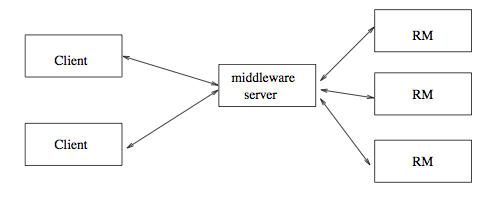
\includegraphics[scale=0.8]{images/image1.png}
\end{center}

Hypothetically, the system can consist of any number of clients greater than one, but it has been tested for 3 clients executing related commands
simultaneously. This concurrency is achieved by synchronizing all reads and writes to the data structures which keep track of customers, flights,
cars, and rooms. Each of the three resource manager servers maintain their own data set consisting of inventory for their respective category. The
middle ware maintains data about all of the customers in the system. For each of the four servers,
this data is stored in the form of a HashTable. Any requests from the client that involve only one
type of booking (either flights, cars, or rooms) are passed on immediately to the appropriate RM. The complete list of these functions is as follows:
\begin{itemize}
 	\item Flight RM: newflight, deleteflight, queryflight, queryflightprice
 	\item Car RM: newcar, deletecar, querycar, querycarprice
 	\item Room RM: newroom, deleteroom, queryroom, queryroomprice
 	\item Middleware: newcustomer, newcustomerid, querycustomer
 	\item Processed in Middleware, accesses RMs as necessary: reserveflight, reservecar, reserveroom,
 	deletecustomer, itinerary
\end{itemize}

What is perhaps worth describing in greater detail is how the Middleware handles the deletecustomer
and the itinerary method. 

In deletecustomer, before a customer is deleted the system needs to
update the resources in each of the RMs to reflect the newly freed resources. To do this,
deletecustomer iterates through all of the reservations related to the customer to be deleted, and
then connects to the appropriate RM for that specific reserved item and calls itemUnReserve.
itemUnReserve then updates the RM's local data structure to reflect these freed resources.

Similarly, in the itinerary method, we cycle through the user's input and call the appropriate RMs
to make the various reservations as required.

Each of the four servers starts their own RMI registry. The RMs use port 7707 and the Middleware
uses port 8807. We intended to use the global RMI registry on teaching on port 1099 but this did not
work. We typically ran the middleware on teaching.cs.mcgill.ca, while the RM servers are run on
lab2-10.cs.mcgill.ca, lab2-11.cs.mcgill.ca, and lab2-12.cs.mcgill.ca. A script was written that can
be run from a fifth machine and remotely starts the four servers on the machines of our choice. This
script also handles killing these processes when it's shut down. We then use a separate script to
run the client on a machine of our choice (typically we use lab2-15.cs.mcgill.ca) as well as another
on another lab machine (to test for concurrency). Most of our testing was done from the client
interface as debugging was not a practical option (given the distributed nature of the system) and
using the output from the servers as reference for what was going on. Every use case we could think
of was tested this way to ensure that everything worked properly.

\newpage
\section{Distributed TCP System}

In terms of design paradigm, the TCP version of our distributed system is in most ways
indistinguishable from the RMI version - we used the same ``division of labour'' here between the
four servers as we did previously. However, under the hood, everything is implemented using sockets
and JSON objects, and so in reality differs a great deal. 

First, the client - in the RMI version, the client simply calls the method of interest; RMI handles
the connection itself. In our TCP system implementation, the client establishes a socket connection
to the middleware server (using socket 1107 in our implementation). The middleware server does not
block client requests. With each new client that wants to connect to the middleware server, the
server creates a separate thread of execution for it. Therefore these clients can send requests
concurrently and the middleware server will execute those requests on separate thread. 

The interaction between the middleware server and the three separate RM server acts similarly. An RM
server can receive requests to perform operations from several different threads of the middleware
server concurrently. Therefore it also creates a separate thread for each connection request from
the middleware server. 

The communication within the sockets is based upon JSON data transfer. When a request is made
either from the client or the middleware, a JSON object is constructed and then passed through the
socket using the DataOutputStream class. JSON responses are passed back from the servers using the
DataOutputStream construction as well. Responses and requests are read using a BufferedReader, and
then parsed for the appropriate and necessary data. 

A notable difference in the TCP implementation
as opposed to RMI is the location of our HashTable objects. Since we want to keep a central
RMHashtable on the middleware or RM servers, the table cannot be constructed in each separate server
handling thread. Instead we create a central table on each server and pass the server class to each
spawned thread in order to allow the thread access to the appropriate information.



\end{document}  
